\chapter{Introduction}

\textbf{Author: Lukas Leskovar}

\vspace{2mm}

\section{The Evolution of Robotics}


Robotic research has always utilized concepts, processes, and methods of different scientific disciplines such as physics, mathematics, and biology to improve application and aid human needs. Because of this industrial, medical and even agricultural sectors have used technologies and products developed by researchers to improve workflows and alleviate employees from performing exhausting tasks. This relationship ranges back to the early ages of information technology in the 1950s and 1960s in which many developments on production robots and Artificial Intelligence (AI) have been made.
Between 1970 and 1990 the public interest in automation and AI has decreased forcing the industry into the so-called AI winter. Despite this recession, research has been continued and the building blocks for another robot boom during the 1990s have been set. Since then the usage of robotic applications has broadened and the industry has proven itself to be a vital aspect of today's economy.

\begin{figure}
	\centering
	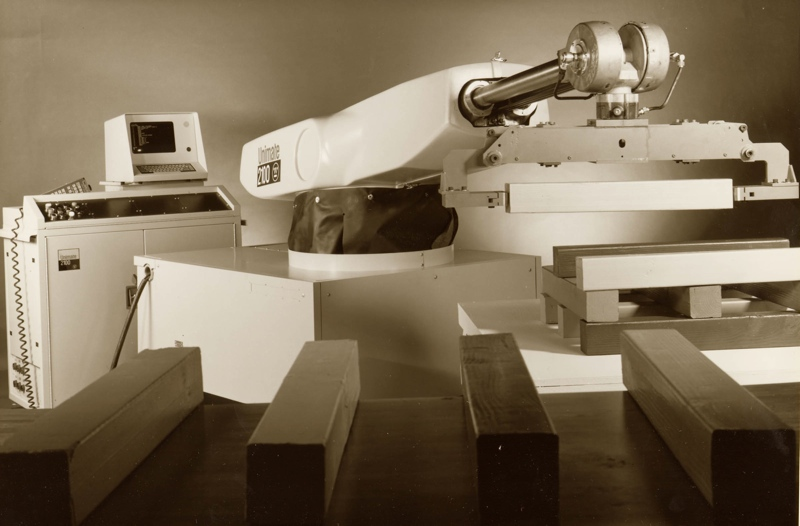
\includegraphics[width=0.7\linewidth]{img/unimate}
	\caption{
		Picture of the first industrial robot. The Unimate developed by George Devol and Joseph Engelbert in 1961 was first used for hot die-casting and welding applications.\protect\footnotemark[1]
	}
	\label{fig:unimate}
\end{figure}
\addtocounter{footnote}{+1}\footnotetext{\cite{unimate}}

\section{Robots with human interaction}
Nowadays the utilization of robots in workplaces has broadened to almost every branch and is accepted by employees and workers. In countries like japan robots are no longer seen as an threat to jobs. 
%noch ein sanfterer Übergang 
Industrial robots are no longer used as simple construction tools, their safety and accuracy has improved so that collaborative robots (Cobots) are capable of working in close cooperation with humans. 
Surgery robots used in the medical sector not only allow for much more accurate procedures but also enable remote specialists to work on patients without having to be in the same hospital. 
In developed countries educational robots are used at school or at home to teach children topics in a playful and interesting way.

\section{Robots in hazardous environments}
Robots do not only serve purpose in a close to user work environment, they also ensure human safety by performing dangerous tasks in unsafe surroundings. 
Remotely controlled robots or drones can be used for inspecting mine shafts, collapsed buildings, pipelines or overhead power poles.
Other applications of such robots are bomb or mine defusion, fire extinction or avalanche rescue.

\section{Autonomous robots}
Implementing a autonomous robot system is a intricate task that proposes many challenging problems for research or development teams. Autonomy requires a system to continuously work in a dynamic environment without external controlling inputs and utilize perceived information about its surroundings in order to adapt to environmental change.\footcite{bekey2005autonomous}
Despite their complexity in development autonomous systems, mobile or stationary, immensely facilitate the execution of a job for the human user.
Such robots can be used to navigate and organize warehouses, construct parts in a assembly line or map large areas for comprehensive calculations.


\section{3D Mapping}

\section{Implementing open-source 3D Mapping}

\section{Technical Objectives}


\filbreak
